% !TEX root = ../intro-stellar-physics.tex

\section{Introduction: Our Sun}

Let's start by considering the star we know best: our sun.  We'll denote the sun with the symbol $\sun$.  From the orbits of the planets we can deduce the mass of the sun from Kepler's laws:
\[
	\Msun = \val{\sci{1.99}{30}}{\kilo\gram}.
\]
This is roughly $10^{6}$ times the mass of the Earth, and is 1\,000 more massive than Jupiter.
Radar ranging of the solar system gives us the mean Earth-Sun distance, which defines the \emph{astronomical unit}
\[
	\val{1}{\AU} = \val{\sci{1.5}{11}}{\meter}.
\]
Knowing this distance and the angular size of the sun then tells us its radius,
\[
	\Rsun = \val{\sci{6.96}{8}}{\meter}.
\]
The sun therefore subtends an angle of about $0.5^{\circ}$ across its diameter.
From measurements of the radiant flux and the distance, we then can infer the sun's radiant power, or luminosity,
\[
	\Lsun = \val{\sci{3.86}{27}}{\watt}.
\]

\begin{exercisebox}[Solar power]
Suppose we wish to replace the Simon power plant with a grid of solar panels. Under ideal conditions (direct light and 100\% efficient panels), how many square meters of solar panels are needed to generate $\val{70}{\Mega\watt}$ ($\val{\sci{70}{6}}{\watt}$)?
\end{exercisebox}

When we observe a star, we collect only a small fraction of this power: if a telescope (or our eye) has a collecting area $\mathcal{A}$ and is a distance $d$ from the star, then it intercepts a fraction $\mathcal{A}/(4\pi d^{2})$ of the star's light.  We call $F = L/(4\pi d^{2})$ the \emph{flux}. The units of flux are $\watt\,\meter^{-2}$.

\begin{exercisebox}[Flux from a distant star]
What would the flux be from a star with $L = \val{0.1}{\Lsun}$ at a distance of $\val{10}{\parsec}$?
Recall that a parsec (pc) is defined by the relation
\[
	\frac{\val{1}{\AU}}{\val{1}{\parsec}} = 1'' = \frac{1}{206265}.
\]
\end{exercisebox}

\section{The nature of light}\label{s.nature-light}

\begin{marginfigure}
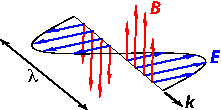
\includegraphics[width=\linewidth]{E-B-free-space}
\caption[The electric force in a light wave]{Schematic of the electric field (blue arrows) and magnetic field (red arrows) for a wave traveling along direction $\bvec{k}$ with wavelength $\lambda$.}
\label{f.light-wave}
\end{marginfigure}
Charges feel an electric force.
When we detect light, what happens at the atomic level is that the charges in our detector (antenna, CCD, eye) feel an electric (and magnetic) force that oscillates with frequency $\nu$. If we could set up a grid of detectors and measure the electric force per unit charge, we would notice a sinusoidal pattern traveling at speed\sidenote{This velocity is exact; the meter is defined in terms of the speed of light.} $c = \val{299\,792\,458}{\meter/\second}$ with a wavelength $\lambda = c/\nu$.  We call this force per charge the electric field $\bvec{E}(\bvec{x},t)$. The \emph{intensity} of the light at our detector is proportional to $|\bvec{E}|^{2} + |\bvec{B}|^{2}$.

Suppose we put a filter in front of our detector that only accepted light in a narrow range of wavelengths $(\lambda,\lambda+\Delta\lambda)$. We would find that energy is deposited into our detector in discrete quanta of magnitude $hc/\lambda = h\nu$\marginnote{The symbol $h = \val{\sci{6.63}{-34}}{\unitstyle{J}\usk\second}$ denotes \emph{Planck's constant}. It sets the scale for quantum mechanics}. We call these quanta \emph{photons}. The light emitted by our sun (or any other source) consists of a huge number of photons distributed over a wide range of wavelengths.

\begin{exercisebox}[Photon flux from the sun]
The sun emits light over a broad range of frequencies, with the peak of this \emph{spectrum} at a wavelength of approximately $\val{500}{\nano\meter}$. Estimate the number of photons from the sun striking $\val{1}{\meter^{2}}$ of Earth each second.
\end{exercisebox}

\section{Intensity and specific flux}
\label{s.intensity-specific-flux}

\begin{marginfigure}[6\baselineskip]
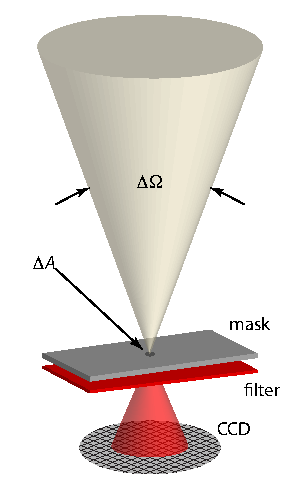
\includegraphics[width=\linewidth]{intensity}
\caption{\label{f.intensity} Schematic of radiative intensity.}
\end{marginfigure}
Take a detector (CCD, your eye, an photographic emulsion) and place in front of the detector a filter that only lets through light with wavelengths in a range $\Delta\lambda$ as before. Then place a mask over the detector with a small pinhole of area $\Delta A$ that restricts the light falling on the detector to fall in a narrow cone of solid angle $\Delta\Omega$ about the normal to the detector (see Fig.~\ref{f.intensity}). Then measure the energy $\Delta E$ incident on the detector in a time $\Delta t$. The quantity
\begin{equation}\label{e.definition-intensity}
I_{\lambda} \equiv \frac{\dif E}{\dif t\,\dif A\,\dif\lambda\,\dif\Omega}
\end{equation}
is known as the \emph{intensity}. It is the basic quantity describing radiation.

In situations in which the wavelength is small (relative to the system in question), light propagates along \emph{rays}. By a ray of light, we mean the light emitted into a small cone of opening solid angle $\dif\Omega$ about a direction $\unitk$. In the absence of any interactions with matter, the intensity is conserved along a ray if both source and receiver are stationary with respect to one another (Exercise~\ref{ex.intensity-conserved}).

\begin{sidebar}[Solid angles]
Imagine that your are at the center of a great sphere of radius $R$, and you shine a light that emits rays into some solid angle. Orient your coordinates so that the rays are traveling along the $z$-axis. The light will illuminate an area
\[ 	A = R^{2}\int_{0}^{2\pi}\int_{0}^{\theta}\sin\theta\,\dif\theta\,\dif\phi. \]
Here $\theta$ is the opening half-angle of the cone. The solid angle into which the light is emitted is $\Omega = A/R^{2}$. Astronomers often express the integral by changing variables to $\mu = \cos\theta$, so that the solid angle is
\[
	\Delta\Omega = \int_{0}^{2\pi}\int_{1-\Delta\mu}^{1}\dif\mu\,\dif\phi.
\]
If we integrate over all angles ($0\le\theta\le\pi$, or $-1\le\mu\le 1$, then we get the area of a sphere, $A = 4\pi R^{2}$.
\end{sidebar}

\begin{exercisebox}[Proof that $I_{\lambda}$ is conserved]
\label{ex.intensity-conserved}
Your friend flashes a light: in a time $\Delta t$ it emits a energy $\Delta E_{\mathrm{emit}}$ in a waveband $\Delta\lambda$. The opening through which the light passes has area $\Delta A_{\mathrm{emit}}$, and the light goes into a cone of opening solid angle $\Delta\Omega_{\mathrm{emit}}$ (see Fig.~\ref{f.intensity-conserved}). Your friend therefore calculates her intensity as
\[	
	I_{\lambda,\mathrm{emit}} = \frac{\Delta E_{\mathrm{emit}}}{\Delta t\,\Delta A_{\mathrm{emit}}\,\Delta\lambda \,\Delta\Omega_{\mathrm{emit}}}.
\]
You stand a distance $d$ ($d^{2}\gg \Delta A_{\mathrm{emit}}, \Delta A_{\mathrm{obs}}$ from your friend with a camera. The aperture on your camera has area $\Delta A_{\mathrm{obs.}}$. Show that the intensity you receive is $I_{\lambda,\mathrm{obs}} = I_{\lambda,\mathrm{emit}}$.
\begin{enumerate}
\item Calculate the incident energy that falls on your camera aperture $\Delta E_{\mathrm{obs}}$.
\item What solid angle $\Delta\Omega_{\mathrm{obs}}$ is subtended by the rays entering the aperture?
\item Now compute your intensity
\[	
	I_{\lambda,\mathrm{obs}} = \frac{\Delta E_{\mathrm{obs}}}{\Delta t\,\Delta A_{\mathrm{obs}}\,\Delta\lambda \,\Delta\Omega_{\mathrm{obs}}}.
\]
and show that this is the same as what your friend calculated.
\end{enumerate}
\end{exercisebox}
\begin{figure*}
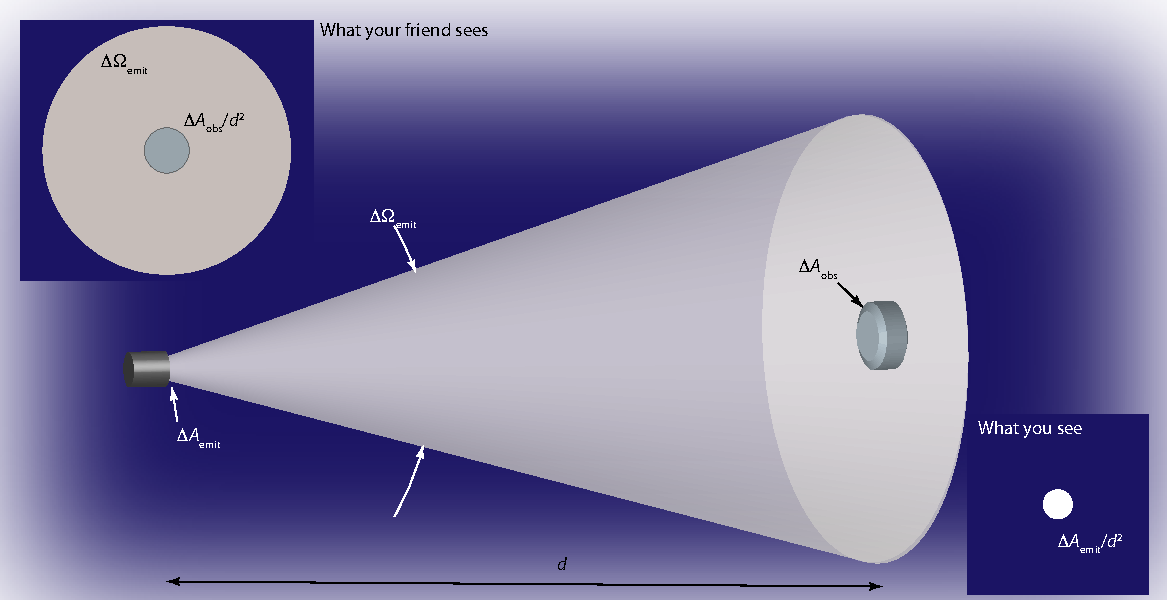
\includegraphics[width=\linewidth]{intensity-conserved}
\caption[Schematic of intensity being constant]{\label{f.intensity-conserved} Schematic for exercise \ref{ex.intensity-conserved}.}
\end{figure*}

To compute the \emph{specific flux} $F_{\lambda}$, we multiply the intensity by $\cos\theta$, where $\theta$ is the angle between the ray and the normal of our area\sidenote{this corrects for the projection of the area} and integrate over angle:
\begin{equation}\label{e.specific-flux}
F_{\lambda} =  \int I_{\lambda}\,\cos\theta\,\sin\theta\,\dif\theta\,\dif\phi.
\end{equation}
The specific flux has dimensions
\[
	[F_{\lambda}] \sim \frac{\textrm{energy}}{\textrm{time}\cdot\textrm{area}\cdot\textrm{wavelength}}.
\]
Astronomers typically use standard filters. For example, the $V$-band filter is centered at $\lambda=\val{551}{\nano\meter}$ and has a width at half-max of $\val{88}{\nano\meter}$. The flux in a particular band, for example $V$ is then
\[
	F_{V} = \int F_{\lambda} \, T(\lambda)\,\dif\lambda;
\]
here $T(\lambda)$ is the \emph{transmission function}, which specifies how much light is let through as a function of wavelength.  The transmission functions for some common UV/optical/IR filters are shown in Figure~\ref{f.UBVRI}.
\begin{figure}
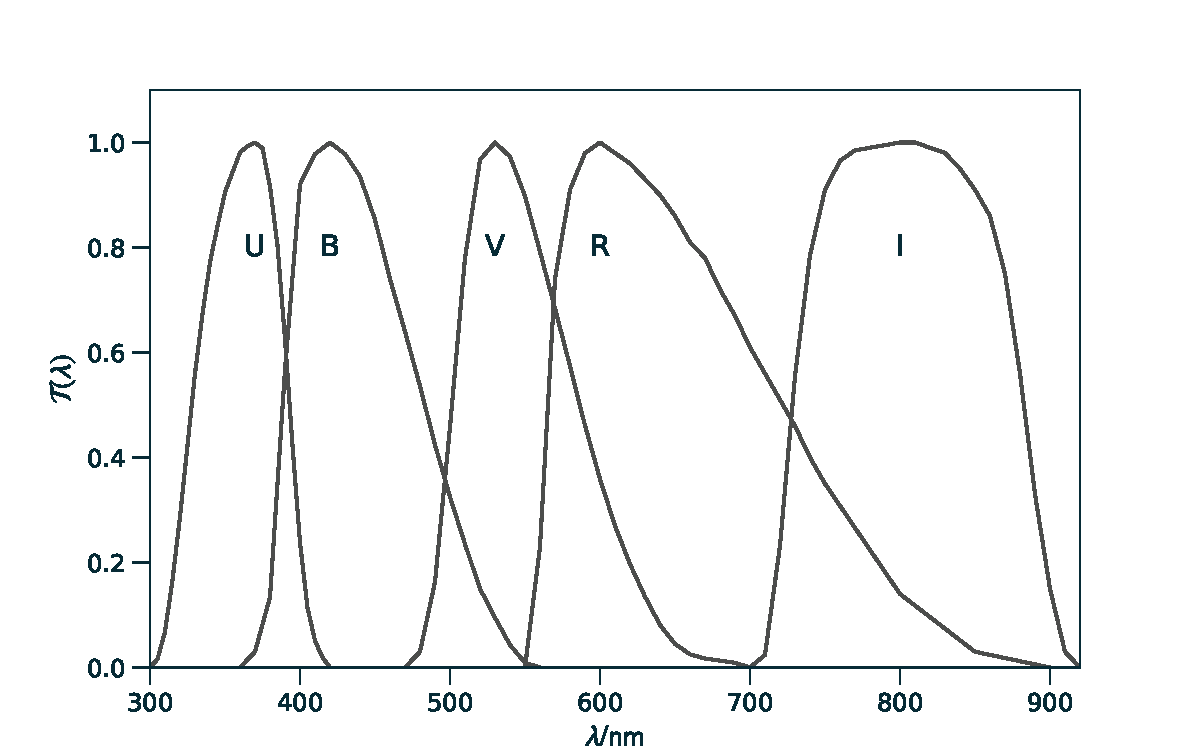
\includegraphics[width=\linewidth]{UBVRI}
\caption[Standard filters]{\label{f.UBVRI} Some standard UV/optical/IR filters. The $T(\lambda)$ are normalized so that $\max(T)=1$.}
\end{figure}

When making observations, it is common to compare the fluxes in a particular band between two stars. Optical astronomers therefore define the \emph{apparent magnitude} as
\marginnote{NB. Throughout this text, $\log\equiv\lg$ denotes $\log_{10}$ and $\ln$ denotes $\log_{e}$.}
\begin{equation}\label{e.apparent-magnitude}
m(A) - m(B) = -2.5\log\left[\frac{F(A)}{F(B)}\right].
\end{equation}
Here $F(A)$ and $F(B)$ are two different measurements of flux (from two different stars, for example) in a particular waveband. It is common to use the label of the waveband in place of $m$.

